%STACK OVERFLOW _ MAY 17
%TIKZ
%BASED ON @Ignasi SOLUTION

%---------------------------------------------------------------------------------------------
%How to draw a rectangle with vertical lines and curved arrows in tikz?
%https://tex.stackexchange.com/questions/370033/how-to-draw-a-rectangle-with-vertical-lines-and-curved-arrows-in-tikz/370080#370080
%---------------------------------------------------------------------------------------------


\documentclass[tikz,border=5pt]{standalone}

\usetikzlibrary{arrows}
%\usetikzlibrary{fit,positioning}
   


\begin{document}

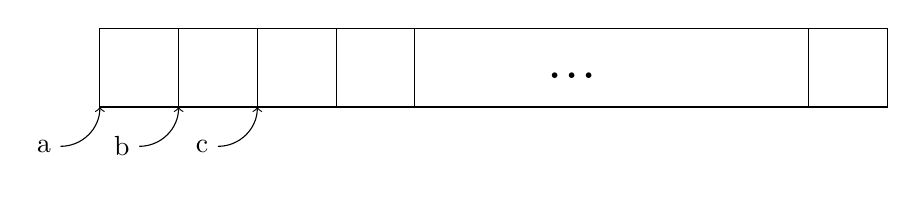
\begin{tikzpicture}[x=-1cm, below, minimum height=2em]
\draw (0,0) rectangle (10,1);
\draw (9,0) -- (9,1);
\draw (8,0) -- (8,1);
\draw (7,0) -- (7,1);

\draw (6,0) -- (6,1) + (-2,-0.25) node[font=\Huge, align=center] {...};

\draw (1,0) -- (1,1);

\draw[<-,->=stealth'] (10.5,-.5cm) node[left] {a} to[out=0, in=-90] +(-.5,.5);
\draw[<-,->=stealth'] (9.5,-.5cm) node[left] {b} to[out=-0, in=-90] ++(-.5,.5) ;
\draw[<-,->=stealth'] (8.5,-.5cm) node[left] {c} to[out=-0, in=-90] ++(-.5,.5);

\end{tikzpicture}

\end{document} 